%%%%%%%%%%%%%%%%%%%%%%%%%%%%%%%%%%%%%%%%%%%%%%%%%%%%%%%%%%%%%%%%%%%%%%%%%%%%%%
%
%  The Institutional Semantic Observatory
%  Part I
%
%%%%%%%%%%%%%%%%%%%%%%%%%%%%%%%%%%%%%%%%%%%%%%%%%%%%%%%%%%%%%%%%%%%%%%%%%%%%%%

\documentclass[aspectratio=169]{beamer}

\usetheme{Madrid}

\usepackage{tikz}
\usetikzlibrary{positioning,arrows.meta,shapes.geometric}

\usepackage{booktabs}
\usepackage{graphicx}
\usepackage{amsmath}
\usepackage{hyperref}

%%%%%%%%%%%%%%%%%%%%%%%%%%%%%%%%%%%%%%%%%%%%%%%%%%%%%%%%%%%%%%%%%%%%%%%%%%%%%%

\definecolor{CNUBlue}{RGB}{0,61,124}

\setbeamercolor{structure}{fg=CNUBlue}
\setbeamercolor{title}{fg=white,bg=CNUBlue}
\setbeamercolor{frametitle}{fg=white,bg=CNUBlue}

%%%%%%%%%%%%%%%%%%%%%%%%%%%%%%%%%%%%%%%%%%%%%%%%%%%%%%%%%%%%%%%%%%%%%%%%%%%%%%

\title{The Institutional Semantic Observatory}
\subtitle{Engineering Information Environments for Explainable Institutional AI}
\author{Edward Brash}
\institute{Christopher Newport University\\School of Engineering and Computing}
\date{\today}

%%%%%%%%%%%%%%%%%%%%%%%%%%%%%%%%%%%%%%%%%%%%%%%%%%%%%%%%%%%%%%%%%%%%%%%%%%%%%%

\begin{document}

%%%%%%%%%%%%%%%%%%%%%%%%%%%%%%%%%%%%%%%%%%%%%%%%%%%%%%%%%%%%%%%%%%%%%%%%%%%%%%

\begin{frame}
\titlepage

\vspace{0.4cm}

\centering
\small

``Information is the resolution of uncertainty.''

\vspace{0.15cm}

--- Claude Shannon
\end{frame}

%%%%%%%%%%%%%%%%%%%%%%%%%%%%%%%%%%%%%%%%%%%%%%%%%%%%%%%%%%%%%%%%%%%%%%%%%%%%%%

\begin{frame}{Universities Have an Information Problem}

Modern universities accumulate enormous quantities of institutional
knowledge.

\vspace{0.4cm}

\begin{columns}[T]

\column{0.50\textwidth}

\begin{itemize}
\item Policies
\item Faculty records
\item Budgets
\item Strategic plans
\item Assessment reports
\item Accreditation documents
\item Meeting minutes
\item Enrollment reports
\item Facilities inventories
\item Historical archives
\end{itemize}

\column{0.50\textwidth}

\Large

A medium-sized university may possess

\vspace{0.3cm}

\centering
{\Huge 15,000+}

documents spanning decades.

\end{columns}

\vspace{0.5cm}

\begin{block}{Observation}
The problem is no longer storing institutional information.

The problem is reasoning over it.
\end{block}

\end{frame}

%%%%%%%%%%%%%%%%%%%%%%%%%%%%%%%%%%%%%%%%%%%%%%%%%%%%%%%%%%%%%%%%%%%%%%%%%%%%%%

\begin{frame}{A Thought Experiment}

Suppose the Provost asks:

\vspace{0.3cm}

\Large

\centering

``Should CNU create a Mechanical Engineering major?''

\normalsize

\vspace{0.5cm}

An experienced dean would begin by gathering evidence.

\begin{itemize}
\item Faculty expertise
\item Laboratory space
\item Equipment
\item ABET implications
\item Budget
\item Enrollment projections
\item Strategic priorities
\end{itemize}

\vspace{0.3cm}

\begin{block}{Observation}
Institutional reasoning begins with evidence gathering.
Only then does reasoning occur.
\end{block}

\end{frame}

%%%%%%%%%%%%%%%%%%%%%%%%%%%%%%%%%%%%%%%%%%%%%%%%%%%%%%%%%%%%%%%%%%%%%%%%%%%%%%

\begin{frame}{The Human Bottleneck}

Imagine giving an experienced dean access to

\vspace{0.2cm}

\Large

\centering

15,000 institutional documents.

\normalsize

\vspace{0.6cm}

The dean faces two fundamental limitations.

\bigskip

\textbf{1. Scale}

Reading the complete corpus could require months or years.

\bigskip

\textbf{2. Recall}

Even with unlimited time,

\emph{which ten documents actually matter?}

\vspace{0.5cm}

\begin{alertblock}{Key Insight}
The bottleneck is not human intelligence.

The bottleneck is locating the appropriate evidence.
\end{alertblock}

\end{frame}

%%%%%%%%%%%%%%%%%%%%%%%%%%%%%%%%%%%%%%%%%%%%%%%%%%%%%%%%%%%%%%%%%%%%%%%%%%%%%%

\begin{frame}{Traditional Retrieval-Augmented Generation (RAG)}

\begin{center}

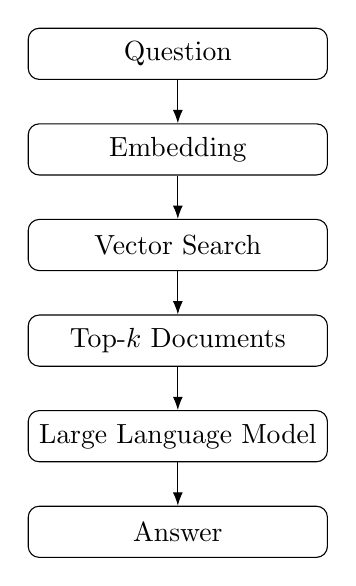
\begin{tikzpicture}[
node distance=0.55cm,
every node/.style={draw,rounded corners,minimum width=3.8cm,
minimum height=0.65cm},
>=Latex]

\node (q) {Question};

\node (e) [below=of q] {Embedding};

\node (v) [below=of e] {Vector Search};

\node (r) [below=of v] {Top-$k$ Documents};

\node (l) [below=of r] {Large Language Model};

\node (a) [below=of l] {Answer};

\draw[->] (q)--(e);
\draw[->] (e)--(v);
\draw[->] (v)--(r);
\draw[->] (r)--(l);
\draw[->] (l)--(a);

\end{tikzpicture}

\end{center}

\vspace{0.3cm}

\begin{block}{Observation}
Retrieval-Augmented Generation dramatically improves factual grounding.

However, the document corpus is largely treated as a passive information source rather than as an engineered information environment.
\end{block}

\end{frame}

%%%%%%%%%%%%%%%%%%%%%%%%%%
%%%%%%%%%%%%%%%%%%%%%%%%%%%%%%%%%%%%%%%%%%%%%%%%%%%%
%
% PART II BEGINS HERE
%
%%%%%%%%%%%%%%%%%%%%%%%%%%%%%%%%%%%%%%%%%%%%%%%%%%%%%%%%%%%%%%%%%%%%%%%%%%%%%%

%%%%%%%%%%%%%%%%%%%%%%%%%%%%%%%%%%%%%%%%%%%%%%%%%%%%%%%%%%%%%%%%%%%%%%%%%%%%%%
%
%  The Institutional Semantic Observatory
%  Part II
%
%%%%%%%%%%%%%%%%%%%%%%%%%%%%%%%%%%%%%%%%%%%%%%%%%%%%%%%%%%%%%%%%%%%%%%%%%%%%%%

\begin{frame}{Where Does Intelligence Live?}

\small

\begin{columns}[T]

\column{0.48\textwidth}

\begin{block}{Conventional AI View}

\begin{itemize}
\item Intelligence resides primarily in the model.
\item Better models should produce better answers.
\item Guardrails constrain model behavior.
\item Trust is placed mainly in the reasoning engine.
\end{itemize}

\end{block}

\column{0.48\textwidth}

\begin{block}{ISO View}

\begin{itemize}
\item Intelligence emerges from the interaction between the model and its information environment.
\item Better information environments produce better evidence.
\item Guardrails shape the conditions under which reasoning occurs.
\item Trust is placed in the complete process.
\end{itemize}

\end{block}

\end{columns}

\vspace{0.45cm}

\begin{alertblock}{Central Thesis}
Reliable institutional reasoning is an emergent property of a
well-engineered information environment.
\end{alertblock}

\end{frame}

%%%%%%%%%%%%%%%%%%%%%%%%%%%%%%%%%%%%%%%%%%%%%%%%%%%%%%%%%%%%%%%%%%%%%%%%%%%%%%

\begin{frame}{Two Philosophies of AI System Design}

\begin{columns}[T]

\column{0.48\textwidth}

\centering
\Large
\textbf{Conventional Approach}

\vspace{0.45cm}

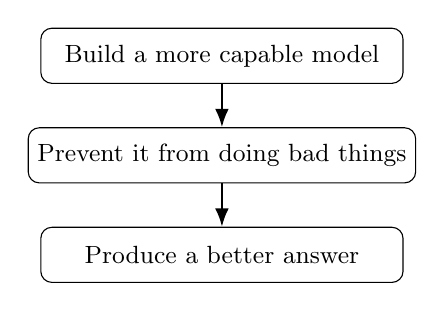
\begin{tikzpicture}[
node distance=0.55cm,
every node/.style={
draw,
rounded corners,
minimum width=4.6cm,
minimum height=0.7cm,
align=center,
font=\small
},
>=Latex
]

\node (model) {Build a more capable model};

\node (prevent) [below=of model]
{Prevent it from doing bad things};

\node (answer) [below=of prevent]
{Produce a better answer};

\draw[->,thick] (model)--(prevent);
\draw[->,thick] (prevent)--(answer);

\end{tikzpicture}

\column{0.48\textwidth}

\centering
\Large
\textbf{ISO Approach}

\vspace{0.45cm}

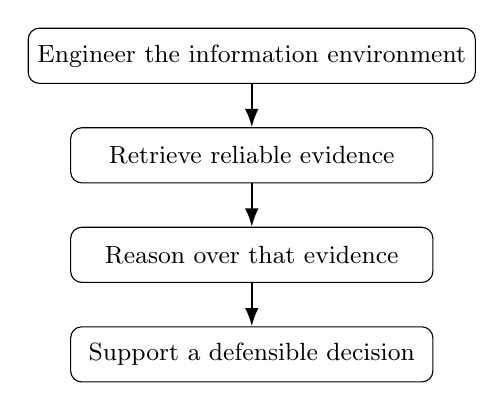
\begin{tikzpicture}[
node distance=0.55cm,
every node/.style={
draw,
rounded corners,
minimum width=4.6cm,
minimum height=0.7cm,
align=center,
font=\small
},
>=Latex
]

\node (environment) {Engineer the information environment};

\node (evidence) [below=of environment]
{Retrieve reliable evidence};

\node (reason) [below=of evidence]
{Reason over that evidence};

\node (decision) [below=of reason]
{Support a defensible decision};

\draw[->,thick] (environment)--(evidence);
\draw[->,thick] (evidence)--(reason);
\draw[->,thick] (reason)--(decision);

\end{tikzpicture}

\end{columns}

\vspace{0.45cm}

\begin{center}
\Large
\textbf{One constrains the actor. The other engineers the environment.}
\end{center}

\end{frame}

%%%%%%%%%%%%%%%%%%%%%%%%%%%%%%%%%%%%%%%%%%%%%%%%%%%%%%%%%%%%%%%%%%%%%%%%%%%%%%

\begin{frame}{Rethinking Guardrails}

The word \emph{guardrail} is often used as though it describes a single
technical mechanism.

\vspace{0.35cm}

In practice, guardrails can be implemented at many layers.

\begin{itemize}
\item Corpus inclusion and exclusion rules
\item Parser validation
\item Provenance requirements
\item Duplicate detection
\item Chunking policy
\item Retrieval constraints
\item Evidence coverage checks
\item Behavioral instructions
\item Human approval requirements
\end{itemize}

\vspace{0.35cm}

\begin{alertblock}{Design Principle}
Guardrails should be implemented at the lowest layer where they can
be made explicit, observable, and auditable.
\end{alertblock}

\end{frame}

%%%%%%%%%%%%%%%%%%%%%%%%%%%%%%%%%%%%%%%%%%%%%%%%%%%%%%%%%%%%%%%%%%%%%%%%%%%%%%

\begin{frame}{The Most Effective Guardrail}

\centering

\vspace{0.5cm}

{\Huge
The most effective guardrail
}

\vspace{0.5cm}

{\Huge
is a well-engineered
}

\vspace{0.5cm}

{\Huge
information environment.
}

\vspace{0.9cm}

\begin{block}{Why?}
A model is less likely to produce an unjustified conclusion when it
receives relevant, diverse, well-provenanced evidence and is explicitly
told when that evidence is incomplete.
\end{block}

\end{frame}

%%%%%%%%%%%%%%%%%%%%%%%%%%%%%%%%%%%%%%%%%%%%%%%%%%%%%%%%%%%%%%%%%%%%%%%%%%%%%%

\begin{frame}{From Information Engineering to Semantic Engineering}

\begin{columns}[T]

\column{0.48\textwidth}

\begin{block}{Information Engineering}

\begin{itemize}
\item Parse files
\item Normalize text
\item Preserve metadata
\item Record provenance
\item Store structured objects
\item Build indexes
\end{itemize}

\end{block}

\column{0.48\textwidth}

\begin{block}{Semantic Engineering}

\begin{itemize}
\item Measure corpus balance
\item Detect dominant documents
\item Identify semantic gaps
\item Monitor retrieval quality
\item Estimate evidence coverage
\item Evaluate reasoning support
\end{itemize}

\end{block}

\end{columns}

\vspace{0.45cm}

\begin{center}
\Large
Information engineering organizes data.

Semantic engineering organizes the conditions for reasoning.
\end{center}

\end{frame}

%%%%%%%%%%%%%%%%%%%%%%%%%%%%%%%%%%%%%%%%%%%%%%%%%%%%%%%%%%%%%%%%%%%%%%%%%%%%%%

\begin{frame}{Knowledge Objects Store Facts}

\Large

\begin{block}{Knowledge Objects}

A knowledge object records what is known about a source without embedding
a conclusion into the source itself.

\end{block}

\vspace{0.35cm}

\small

Typical fields include

\begin{itemize}
\item source path
\item title
\item parser
\item timestamps
\item document type
\item normalized text
\item semantic chunks
\item provenance
\item extraction metadata
\item quality indicators
\end{itemize}

\vspace{0.3cm}

\begin{alertblock}{Architectural Principle}
Knowledge objects store facts.
\end{alertblock}

\end{frame}

%%%%%%%%%%%%%%%%%%%%%%%%%%%%%%%%%%%%%%%%%%%%%%%%%%%%%%%%%%%%%%%%%%%%%%%%%%%%%%

\begin{frame}{Services Derive Meaning}

\Large

\begin{block}{Services}

Services operate over knowledge objects to derive context-dependent meaning.

\end{block}

\vspace{0.35cm}

\small

Examples include

\begin{itemize}
\item retrieval
\item reranking
\item evidence synthesis
\item corpus diagnostics
\item scenario analysis
\item decision brief generation
\item conflict detection
\item confidence assessment
\end{itemize}

\vspace{0.3cm}

\begin{alertblock}{Architectural Principle}
Services derive meaning.
\end{alertblock}

\end{frame}

%%%%%%%%%%%%%%%%%%%%%%%%%%%%%%%%%%%%%%%%%%%%%%%%%%%%%%%%%%%%%%%%%%%%%%%%%%%%%%

\begin{frame}{The ISO Pipeline}

\centering

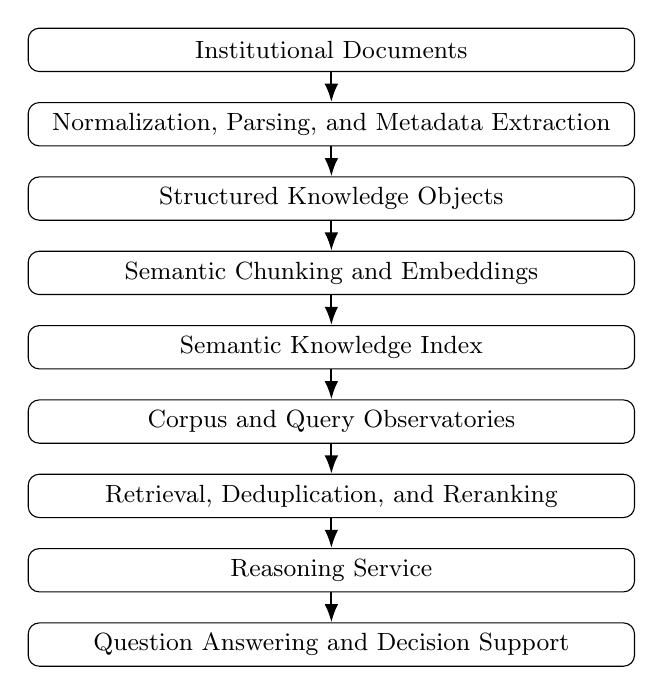
\begin{tikzpicture}[
node distance=0.38cm,
every node/.style={
draw,
rounded corners,
minimum width=7.7cm,
minimum height=0.55cm,
align=center,
font=\small,
inner sep=3pt
},
>=Latex
]

\node (docs) {Institutional Documents};

\node (norm) [below=of docs]
{Normalization, Parsing, and Metadata Extraction};

\node (objects) [below=of norm]
{Structured Knowledge Objects};

\node (chunks) [below=of objects]
{Semantic Chunking and Embeddings};

\node (index) [below=of chunks]
{Semantic Knowledge Index};

\node (observe) [below=of index]
{Corpus and Query Observatories};

\node (retrieve) [below=of observe]
{Retrieval, Deduplication, and Reranking};

\node (reason) [below=of retrieve]
{Reasoning Service};

\node (output) [below=of reason]
{Question Answering and Decision Support};

\draw[->,thick] (docs)--(norm);
\draw[->,thick] (norm)--(objects);
\draw[->,thick] (objects)--(chunks);
\draw[->,thick] (chunks)--(index);
\draw[->,thick] (index)--(observe);
\draw[->,thick] (observe)--(retrieve);
\draw[->,thick] (retrieve)--(reason);
\draw[->,thick] (reason)--(output);

\end{tikzpicture}

\end{frame}

%%%%%%%%%%%%%%%%%%%%%%%%%%%%%%%%%%%%%%%%%%%%%%%%%%%%%%%%%%%%%%%%%%%%%%%%%%%%%%
%
% PART III BEGINS HERE
%
%%%%%%%%%%%%%%%%%%%%%%%%%%%%%%%%%%%%%%%%%%%%%%%%%%%%%%%%%%%%%%%%%%%%%%%%%%%%%%

%%%%%%%%%%%%%%%%%%%%%%%%%%%%%%%%%%%%%%%%%%%%%%%%%%%%%%%%%%%%%%%%%%%%%%%%%%%%%%
%
%  The Institutional Semantic Observatory
%  Part III
%
%%%%%%%%%%%%%%%%%%%%%%%%%%%%%%%%%%%%%%%%%%%%%%%%%%%%%%%%%%%%%%%%%%%%%%%%%%%%%%

\begin{frame}{The Semantic Ecosystem}

A corpus is not merely a collection of files.

\vspace{0.35cm}

It is an information environment with structure.

\vspace{0.45cm}

\begin{columns}[T]

\column{0.48\textwidth}

\begin{block}{Healthy Properties}

\begin{itemize}
\item Diversity
\item Balance
\item Provenance
\item Connectivity
\item Resilience
\item Observability
\item Evolution over time
\end{itemize}

\end{block}

\column{0.48\textwidth}

\begin{block}{Pathologies}

\begin{itemize}
\item Dominant documents
\item Duplicates
\item Corrupted files
\item Stale knowledge
\item Semantic islands
\item Missing regions
\item Parser failures
\end{itemize}

\end{block}

\end{columns}

\vspace{0.45cm}

\begin{alertblock}{Working Definition}
A semantic ecosystem is the structured information environment
within which retrieval and reasoning occur.
\end{alertblock}

\end{frame}

%%%%%%%%%%%%%%%%%%%%%%%%%%%%%%%%%%%%%%%%%%%%%%%%%%%%%%%%%%%%%%%%%%%%%%%%%%%%%%

\begin{frame}{Why an Observatory?}

In every mature scientific system, instrumentation is used to monitor
the health of the environment in which inference occurs.

\vspace{0.45cm}

\begin{columns}[T]

\column{0.31\textwidth}

\begin{block}{Experimental Physics}
\centering
Detector monitoring

Calibration

Efficiency

Systematics
\end{block}

\column{0.31\textwidth}

\begin{block}{Ecology}
\centering
Population density

Diversity

Fragmentation

Resilience
\end{block}

\column{0.31\textwidth}

\begin{block}{ISO}
\centering
Corpus balance

Parser health

Retrieval quality

Evidence support
\end{block}

\end{columns}

\vspace{0.55cm}

\begin{center}
\Large
The observatory is not an auxiliary dashboard.

It is part of the reasoning infrastructure.
\end{center}

\end{frame}

%%%%%%%%%%%%%%%%%%%%%%%%%%%%%%%%%%%%%%%%%%%%%%%%%%%%%%%%%%%%%%%%%%%%%%%%%%%%%%

\begin{frame}{The Corpus Observatory}

\begin{columns}[T]

\column{0.42\textwidth}

The current observatory measures global properties of the corpus.

\vspace{0.3cm}

\begin{itemize}
\item Document count
\item Total semantic chunks
\item Chunks per document
\item File-type distribution
\item Parser distribution
\item Folder distribution
\item Dominance metrics
\item Gini coefficient
\item Largest documents
\item Outlier detection
\end{itemize}

\column{0.56\textwidth}

\centering

\fbox{
\parbox[c][5.2cm][c]{0.95\linewidth}{
\centering

\vspace{1.7cm}

\Large
Semantic Observatory Screenshot

\vspace{0.25cm}

\normalsize
Insert corpus-health image here

\vspace{1.7cm}
}
}

\end{columns}

\end{frame}

%%%%%%%%%%%%%%%%%%%%%%%%%%%%%%%%%%%%%%%%%%%%%%%%%%%%%%%%%%%%%%%%%%%%%%%%%%%%%%

\begin{frame}{What Does the Gini Coefficient Measure?}

The Gini coefficient measures how unevenly semantic chunks are
distributed across documents.

\vspace{0.5cm}

\begin{columns}[T]

\column{0.47\textwidth}

\begin{block}{Low Gini}

\begin{itemize}
\item Information is distributed relatively evenly.
\item No small group of documents dominates the corpus.
\item Retrieval is less likely to be overwhelmed by a few sources.
\end{itemize}

\end{block}

\column{0.47\textwidth}

\begin{block}{High Gini}

\begin{itemize}
\item A small number of documents contain a large fraction of all chunks.
\item Large or duplicated files may dominate retrieval.
\item Corpus health may require investigation.
\end{itemize}

\end{block}

\end{columns}

\vspace{0.5cm}

\begin{alertblock}{Important}
The Gini coefficient is not a score to maximize or minimize.

It is a diagnostic indicator of corpus structure.
\end{alertblock}

\end{frame}

%%%%%%%%%%%%%%%%%%%%%%%%%%%%%%%%%%%%%%%%%%%%%%%%%%%%%%%%%%%%%%%%%%%%%%%%%%%%%%

\begin{frame}{A Real Corpus Pathology}

One spreadsheet initially generated approximately

\vspace{0.2cm}

\begin{center}
{\Huge 50,000}
\end{center}

semantic chunks.

\vspace{0.25cm}

The spreadsheet appeared modest when viewed normally.

However, several corrupted rows extended across thousands of columns
and repeated the same values many times.

\vspace{0.45cm}

\begin{block}{What the Observatory Revealed}

\begin{itemize}
\item Extreme document dominance
\item Inflated chunk counts
\item Distorted corpus statistics
\item Wasted embedding and indexing resources
\item Increased risk of retrieval contamination
\end{itemize}

\end{block}

\vspace{0.3cm}

After repairing the source file, the normalized document became
commensurate with its actual information content.

\end{frame}

%%%%%%%%%%%%%%%%%%%%%%%%%%%%%%%%%%%%%%%%%%%%%%%%%%%%%%%%%%%%%%%%%%%%%%%%%%%%%%

\begin{frame}{From Corpus Health to Query Health}

The Corpus Observatory asks:

\vspace{0.25cm}

\begin{center}
\Large
Is the overall information environment healthy?
\end{center}

\vspace{0.55cm}

The next phase asks a more local question:

\vspace{0.25cm}

\begin{center}
\Large
How well supported is this particular reasoning task?
\end{center}

\vspace{0.55cm}

\begin{block}{Query Observatory}
A Query Observatory evaluates the state of the information
environment relative to a specific question before the final
reasoning step occurs.
\end{block}

\end{frame}

%%%%%%%%%%%%%%%%%%%%%%%%%%%%%%%%%%%%%%%%%%%%%%%%%%%%%%%%%%%%%%%%%%%%%%%%%%%%%%

\begin{frame}{Local Information Density}

Each query occupies a location in semantic space.

\vspace{0.4cm}

Some regions are densely populated with relevant evidence.

Other regions contain little or no institutional information.

\vspace{0.5cm}

\begin{columns}[T]

\column{0.48\textwidth}

\begin{block}{Dense Region}

\begin{itemize}
\item Many nearby chunks
\item Small nearest-neighbor distances
\item Stable retrieval neighborhoods
\item Strong semantic support
\end{itemize}

\end{block}

\column{0.48\textwidth}

\begin{block}{Sparse Region}

\begin{itemize}
\item Few nearby chunks
\item Large nearest-neighbor distances
\item Unstable retrieval
\item Greater risk of unsupported inference
\end{itemize}

\end{block}

\end{columns}

\vspace{0.45cm}

\begin{alertblock}{Working Hypothesis}
Hallucination risk may increase when a query lies in a region of low
local information density.
\end{alertblock}

\end{frame}

%%%%%%%%%%%%%%%%%%%%%%%%%%%%%%%%%%%%%%%%%%%%%%%%%%%%%%%%%%%%%%%%%%%%%%%%%%%%%%

\begin{frame}{Evidence Diversity}

Ten retrieved chunks do not necessarily represent ten independent
pieces of evidence.

\vspace{0.35cm}

The system may return

\begin{itemize}
\item ten chunks from the same document,
\item multiple copies of the same catalog,
\item several nearly identical forms,
\item or genuinely diverse evidence from independent sources.
\end{itemize}

\vspace{0.45cm}

\begin{block}{Possible Diversity Measures}

\begin{itemize}
\item Unique documents
\item Unique folders
\item Unique document types
\item Unique authors or offices
\item Unique years
\item Semantic entropy
\item Source-category balance
\end{itemize}

\end{block}

\vspace{0.35cm}

Diverse evidence does not guarantee correctness, but it reduces the
chance that one source silently controls the conclusion.

\end{frame}

%%%%%%%%%%%%%%%%%%%%%%%%%%%%%%%%%%%%%%%%%%%%%%%%%%%%%%%%%%%%%%%%%%%%%%%%%%%%%%

\begin{frame}{Retrieval Stability}

A well-supported question should retrieve similar evidence under small
changes in wording.

\vspace{0.4cm}

For example:

\begin{itemize}
\item Mechanical Engineering major
\item Mechanical Engineering program
\item ME degree
\item New undergraduate engineering program
\end{itemize}

\vspace{0.45cm}

\begin{block}{High Stability}
Small query perturbations retrieve substantially overlapping evidence.
\end{block}

\begin{block}{Low Stability}
Minor wording changes produce very different retrieval neighborhoods.
\end{block}

\vspace{0.35cm}

\begin{alertblock}{Interpretation}
Low retrieval stability is evidence that the semantic neighborhood is
poorly defined or weakly supported.
\end{alertblock}

\end{frame}

%%%%%%%%%%%%%%%%%%%%%%%%%%%%%%%%%%%%%%%%%%%%%%%%%%%%%%%%%%%%%%%%%%%%%%%%%%%%%%

\begin{frame}{Evidence Completeness}

A strategic question often requires evidence from multiple domains.

\vspace{0.4cm}

For a proposed academic program, relevant domains may include

\begin{itemize}
\item curriculum
\item faculty expertise
\item enrollment demand
\item budget
\item facilities
\item equipment
\item accreditation
\item strategic alignment
\end{itemize}

\vspace{0.45cm}

\begin{block}{Coverage Question}
Did retrieval find evidence for all required domains, or only a subset?
\end{block}

\vspace{0.35cm}

A high-quality answer may still be impossible when several essential
evidence domains are missing.

\end{frame}

%%%%%%%%%%%%%%%%%%%%%%%%%%%%%%%%%%%%%%%%%%%%%%%%%%%%%%%%%%%%%%%%%%%%%%%%%%%%%%

\begin{frame}{The Query Observatory}

\small

\begin{columns}[T]

\column{0.52\textwidth}

\begin{block}{Example Question}

What resources would be required to launch a Mechanical Engineering
major?

\end{block}

\vspace{0.2cm}

\begin{tabular}{lr}

Local information density & 9.4 / 10 \\

Evidence diversity & 8.8 / 10 \\

Provenance quality & 9.1 / 10 \\

Retrieval stability & 8.4 / 10 \\

Evidence completeness & 7.6 / 10 \\

\end{tabular}

\vspace{0.4cm}

\begin{alertblock}{Expected Reasoning Reliability}
High
\end{alertblock}

\column{0.44\textwidth}

\begin{block}{Inspectable Diagnostics}

\begin{itemize}
\item Nearest-neighbor distances
\item Retrieved-document overlap
\item Source-category entropy
\item Parser quality
\item Provenance completeness
\item Domain coverage
\item Evidence conflicts
\end{itemize}

\end{block}

\end{columns}

\end{frame}

%%%%%%%%%%%%%%%%%%%%%%%%%%%%%%%%%%%%%%%%%%%%%%%%%%%%%%%%%%%%%%%%%%%%%%%%%%%%%%
%
% PART IV BEGINS HERE
%
%%%%%%%%%%%%%%%%%%%%%%%%%%%%%%%%%%%%%%%%%%%%%%%%%%%%%%%%%%%%%%%%%%%%%%%%%%%%%%

%%%%%%%%%%%%%%%%%%%%%%%%%%%%%%%%%%%%%%%%%%%%%%%%%%%%%%%%%%%%%%%%%%%%%%%%%%%%%%
%
%  The Institutional Semantic Observatory
%  Part IV
%
%%%%%%%%%%%%%%%%%%%%%%%%%%%%%%%%%%%%%%%%%%%%%%%%%%%%%%%%%%%%%%%%%%%%%%%%%%%%%%

\begin{frame}{Case Study I: Decision Support}

Question:

\vspace{0.2cm}

\Large

\centering

Should CNU create a Mechanical Engineering major?

\normalsize

\vspace{0.5cm}

ISO does not begin by producing an answer.

Instead it asks:

\begin{itemize}
\item What evidence exists?
\item Is the evidence sufficient?
\item What evidence is missing?
\item How reliable is the evidence?
\end{itemize}

\vspace{0.4cm}

\begin{block}{Decision Support}
ISO assists human decision makers by assembling,
organizing, evaluating, and explaining evidence.

The decision itself remains a human responsibility.
\end{block}

\end{frame}

%%%%%%%%%%%%%%%%%%%%%%%%%%%%%%%%%%%%%%%%%%%%%%%%%%%%%%%%%%%%%%%%%%%%%%%%%%%%%%

\begin{frame}{Case Study II: Epistemic Humility}

Question:

\vspace{0.2cm}

\Large

\centering

Should CNU eliminate the French major?

\normalsize

\vspace{0.5cm}

ISO retrieved curriculum documents,
catalogs,
planning forms,
and language placement information.

\vspace{0.3cm}

However, the system explicitly reported missing evidence.

\begin{itemize}
\item Enrollment history
\item Budget
\item Faculty workload
\item Strategic planning
\item Program review
\end{itemize}

\vspace{0.4cm}

\begin{alertblock}{Correct Conclusion}
The available evidence is insufficient to support
a recommendation.

Additional information is required.
\end{alertblock}

\end{frame}

%%%%%%%%%%%%%%%%%%%%%%%%%%%%%%%%%%%%%%%%%%%%%%%%%%%%%%%%%%%%%%%%%%%%%%%%%%%%%%

\begin{frame}{A Scientist, Not a Chatbot}

Traditional chatbots attempt to answer nearly every question.

\vspace{0.5cm}

ISO attempts something different.

\vspace{0.5cm}

\begin{columns}[T]

\column{0.47\textwidth}

\begin{block}{Scientist}

\begin{itemize}
\item Examine evidence
\item State assumptions
\item Report uncertainty
\item Explain conclusions
\item Identify missing data
\end{itemize}

\end{block}

\column{0.47\textwidth}

\begin{block}{Desired ISO Behavior}

\begin{itemize}
\item Retrieve evidence
\item Measure evidence quality
\item Synthesize findings
\item Explain reasoning
\item Recommend follow-up
\end{itemize}

\end{block}

\end{columns}

\vspace{0.5cm}

\begin{center}
\Large

The objective is not artificial certainty.

The objective is trustworthy reasoning.

\end{center}

\end{frame}

%%%%%%%%%%%%%%%%%%%%%%%%%%%%%%%%%%%%%%%%%%%%%%%%%%%%%%%%%%%%%%%%%%%%%%%%%%%%%%

\begin{frame}{Toward a Science of Institutional Reasoning}

We believe that institutional reasoning can become an
observable and measurable engineering discipline.

\vspace{0.45cm}

Future observatory metrics may include

\begin{itemize}
\item Local information density
\item Evidence diversity
\item Evidence completeness
\item Provenance quality
\item Retrieval stability
\item Semantic conflict detection
\item Expected reasoning reliability
\item Longitudinal corpus evolution
\end{itemize}

\vspace{0.45cm}

These are properties of the
\textbf{information environment},
not merely of the language model.

\end{frame}

%%%%%%%%%%%%%%%%%%%%%%%%%%%%%%%%%%%%%%%%%%%%%%%%%%%%%%%%%%%%%%%%%%%%%%%%%%%%%%

\begin{frame}{Research Directions}

\begin{columns}[T]

\column{0.48\textwidth}

\textbf{Engineering}

\begin{itemize}
\item Knowledge objects
\item Ontology construction
\item Corpus observatories
\item Query observatories
\item Provenance graphs
\item Retrieval benchmarking
\item Information quality metrics
\end{itemize}

\column{0.48\textwidth}

\textbf{Scientific Questions}

\begin{itemize}
\item Does local information density predict answer quality?
\item Does evidence diversity reduce hallucinations?
\item How should reasoning reliability be estimated?
\item Which observatory metrics best predict trustworthy decisions?
\item Can semantic ecosystems be optimized?
\end{itemize}

\end{columns}

\end{frame}

%%%%%%%%%%%%%%%%%%%%%%%%%%%%%%%%%%%%%%%%%%%%%%%%%%%%%%%%%%%%%%%%%%%%%%%%%%%%%%

\begin{frame}{The Emerging Architecture}

\centering

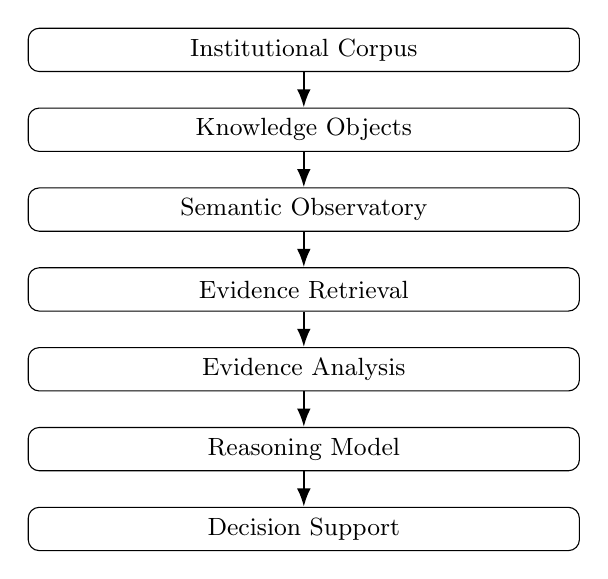
\begin{tikzpicture}[
node distance=0.45cm,
every node/.style={
draw,
rounded corners,
minimum width=7cm,
minimum height=0.55cm,
align=center,
font=\small
},
>=Latex
]

\node (corpus){Institutional Corpus};

\node (objects)[below=of corpus]{Knowledge Objects};

\node (observatory)[below=of objects]{Semantic Observatory};

\node (retrieval)[below=of observatory]{Evidence Retrieval};

\node (analysis)[below=of retrieval]{Evidence Analysis};

\node (reasoning)[below=of analysis]{Reasoning Model};

\node (support)[below=of reasoning]{Decision Support};

\draw[->,thick](corpus)--(objects);
\draw[->,thick](objects)--(observatory);
\draw[->,thick](observatory)--(retrieval);
\draw[->,thick](retrieval)--(analysis);
\draw[->,thick](analysis)--(reasoning);
\draw[->,thick](reasoning)--(support);

\end{tikzpicture}

\vspace{0.45cm}

\Large

Engineer the environment.

Reliable reasoning follows.

\end{frame}

%%%%%%%%%%%%%%%%%%%%%%%%%%%%%%%%%%%%%%%%%%%%%%%%%%%%%%%%%%%%%%%%%%%%%%%%%%%%%%

\begin{frame}{Summary}

\begin{enumerate}

\item Institutional reasoning begins with evidence.

\vspace{0.15cm}

\item Human intelligence is limited primarily by scale and recall.

\vspace{0.15cm}

\item Retrieval-Augmented Generation is a major advance,
but the information environment itself deserves engineering.

\vspace{0.15cm}

\item Knowledge objects store facts.

\vspace{0.15cm}

\item Services derive meaning.

\vspace{0.15cm}

\item Corpus and Query Observatories make reasoning
observable, measurable, and explainable.

\vspace{0.15cm}

\item Reliable institutional reasoning is an emergent property
of a well-engineered information environment.

\end{enumerate}

\end{frame}

%%%%%%%%%%%%%%%%%%%%%%%%%%%%%%%%%%%%%%%%%%%%%%%%%%%%%%%%%%%%%%%%%%%%%%%%%%%%%%

\begin{frame}

\centering

\vspace{1.3cm}

{\Huge Questions?}

\vspace{1.0cm}

{\Large Discussion}

\vspace{1.5cm}

\Large

\textbf{The Institutional Semantic Observatory}

\vspace{0.25cm}

Engineering Information Environments for Explainable Institutional AI

\end{frame}

%%%%%%%%%%%%%%%%%%%%%%%%%%%%%%%%%%%%%%%%%%%%%%%%%%%%%%%%%%%%%%%%%%%%%%%%%%%%%%

\end{document}
